\section{Аналитический расчет взаимодействия диполей}
Рассмотрим теперь взаимодействие двух диполей без приближения ближнего поля (\ref{eq:f_Taylor}). Так как поляризация первого диполя создает электрическое поле в первом диполе, а поляризация второго диполя --- в первом, и зная соотношение между электрическим полем $ \textbf{E} (r) $ и поляризацией $ \textbf{P} $ через тензор диэлектрической восприимчивости $ \chi $, получим системы линейных однородных алгебраических уравнений относительно поляризации $ \textbf{P} (i) $, где $ i $ --- i-ый диполь:
\begin{subequations}
\begin{gather}
\frac{\textbf{P}(1)}{\alpha} - \chi \textbf{P}(2) = 0, \label{eq:linear_eq_P1} \\
\chi \textbf{P}(1) -  \frac{\textbf{P}(2)}{\alpha} = 0, \label{eq:linear_eq_P2} 
\end{gather}
\end{subequations}
где $ \alpha $ --- поляризуемость, определяемая формулой (\ref{eq:polarizability_dipole}), а произведение диэлектрической восприимчивости на поляризацию определяется в общем случае формулой
\begin{multline}
\chi \textbf{P} = \exp (\imath k r) \Bigg( \left( \frac{P_x}{r} \left( k^2 + \imath \frac{k}{r} - \frac{1}{r^2} \right) \right) \mathbf{e_x} + \left( \frac{P_y}{r} \left( k^2 + \imath \frac{k}{r} - \frac{1}{r^2} \right) \right) \mathbf{e_y} + \\
+ \left( \frac{P_z}{r} \left( - \imath \frac{2 k}{r} + \frac{2}{r^2} \right) \right) \mathbf{e_z} \Bigg).
\label{eq:2D_susceptibility}
\end{multline}
Рассмотрим анизотропный тензор поляризуемости $ \alpha = \alpha_{xx} \neq 0 $. Тогда в уравнении (\ref{eq:2D_susceptibility}) остается слагаемое с $ \mathbf{e_x} $, а остальные зануляются. Представим систему уравнений (\ref{eq:linear_eq_P1}, \ref{eq:linear_eq_P2}) в виде матрицы и найдем через ее собственные значения резонансные частоты $ \omega_s $ и $ \omega_a $, которые относятся к симметричному и антисимметричному случаю взаимодействия диполей. В ходе анализа был написан скрипт в программном пакете MATHEMATICA, который вычислял положения резонансов $ \lambda_s $ и $ \lambda_a $. Далее была исследована зависимость положения резонансных длин волн $ \lambda_s $ и $ \lambda_a $ от расстояния между диполями. Для этого выбирались определенное расстояние $ d $ между диполями от значения $ d = $ 50 нм до $ d = $ 400 нм с шагом 1 нм и численно находились резонансные длины волн  $ \lambda_s $ и $ \lambda_a $. На рис.~\ref{img:2D_res} показана зависимость положения резонанснов ЛПП $ \lambda_s $ и $ \lambda_a $ от расстояния между диполями. Видно, что в отличие от зависимости в ближнепольном приближении (рис.~\ref{img:semianalytical_dd}) появляются осцилляции, связанные с влиянием дальнего поля.
\begin{figure}
\center{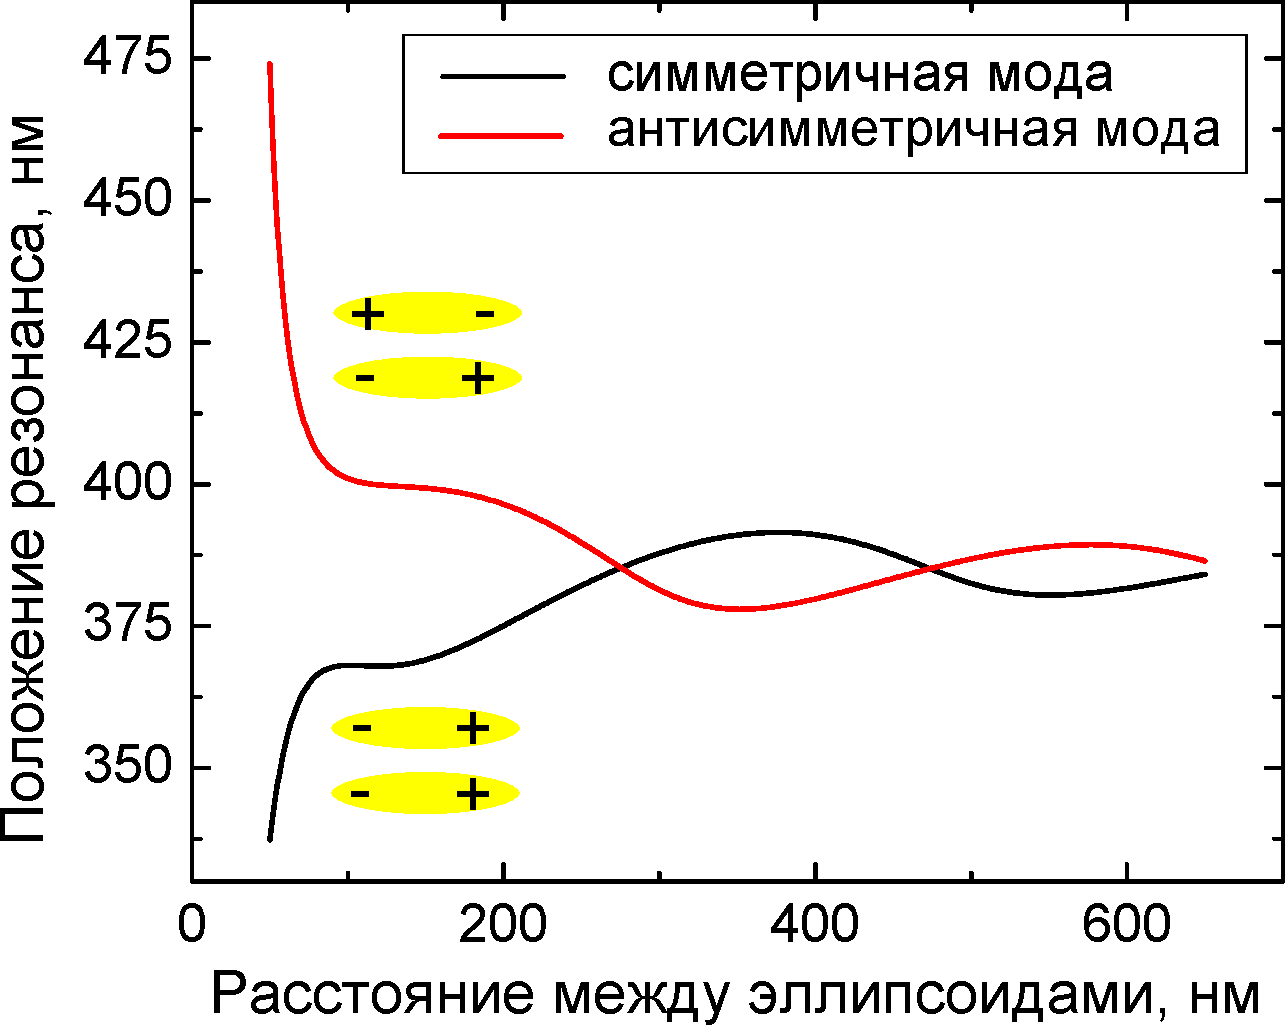
\includegraphics[width=0.5\linewidth]{img/analytics/res_dd.pdf}}
\caption{Зависимость положения симметричного $ \lambda_s $ и антисимметричного $ \lambda_a $ резонанса от расстояния $ d $ между диполями. Вставки --- мгновенное распределение зарядов в случае симметричной и антисимметричной моды.}
\label{img:2D_res}
\end{figure}
Данные осцилляции являются "паразитными" для верхней границы применимости димера в качестве плазмонной линейки. Они связаны с тем, что в отличии от формулы (\ref{eq:wl_dipole}), в которой учитывалась только ближнепольная компонента поля $ \frac{1}{r^2} $, учитывается и влияние множителей $ \frac{k}{r} $ , $ k^2 $, а экспонента не раскладывается в ряд Тейлора по малому параметру $ kr $.

%Абзац -- сравнение аналитического решения и численного расчета FDTD
Далее рассматривались эллипсоиды с различной длиной. По формуле (\ref{eq:Lfactor}) рассчитывался фактор деполяризации данного эллипсоида, а по формуле (\ref{eq:polarizabilityEllip}) --- его поляризуемость. Для эллипсоидов с длиной $ a = $ 100, 150, 200 и 300 нм рассчитывалась зависимость положения резонансной длины волны ЛПП симметричной моды от расстояния между эллипсоидами. Полученные данные сравнивались с численными расчетами для $ \pi $-димера золотых наностержней такой же длины с граничными условиями PML на рис.~\ref{img:res1_analytic_FDTD}.
\begin{figure}[t]
\center{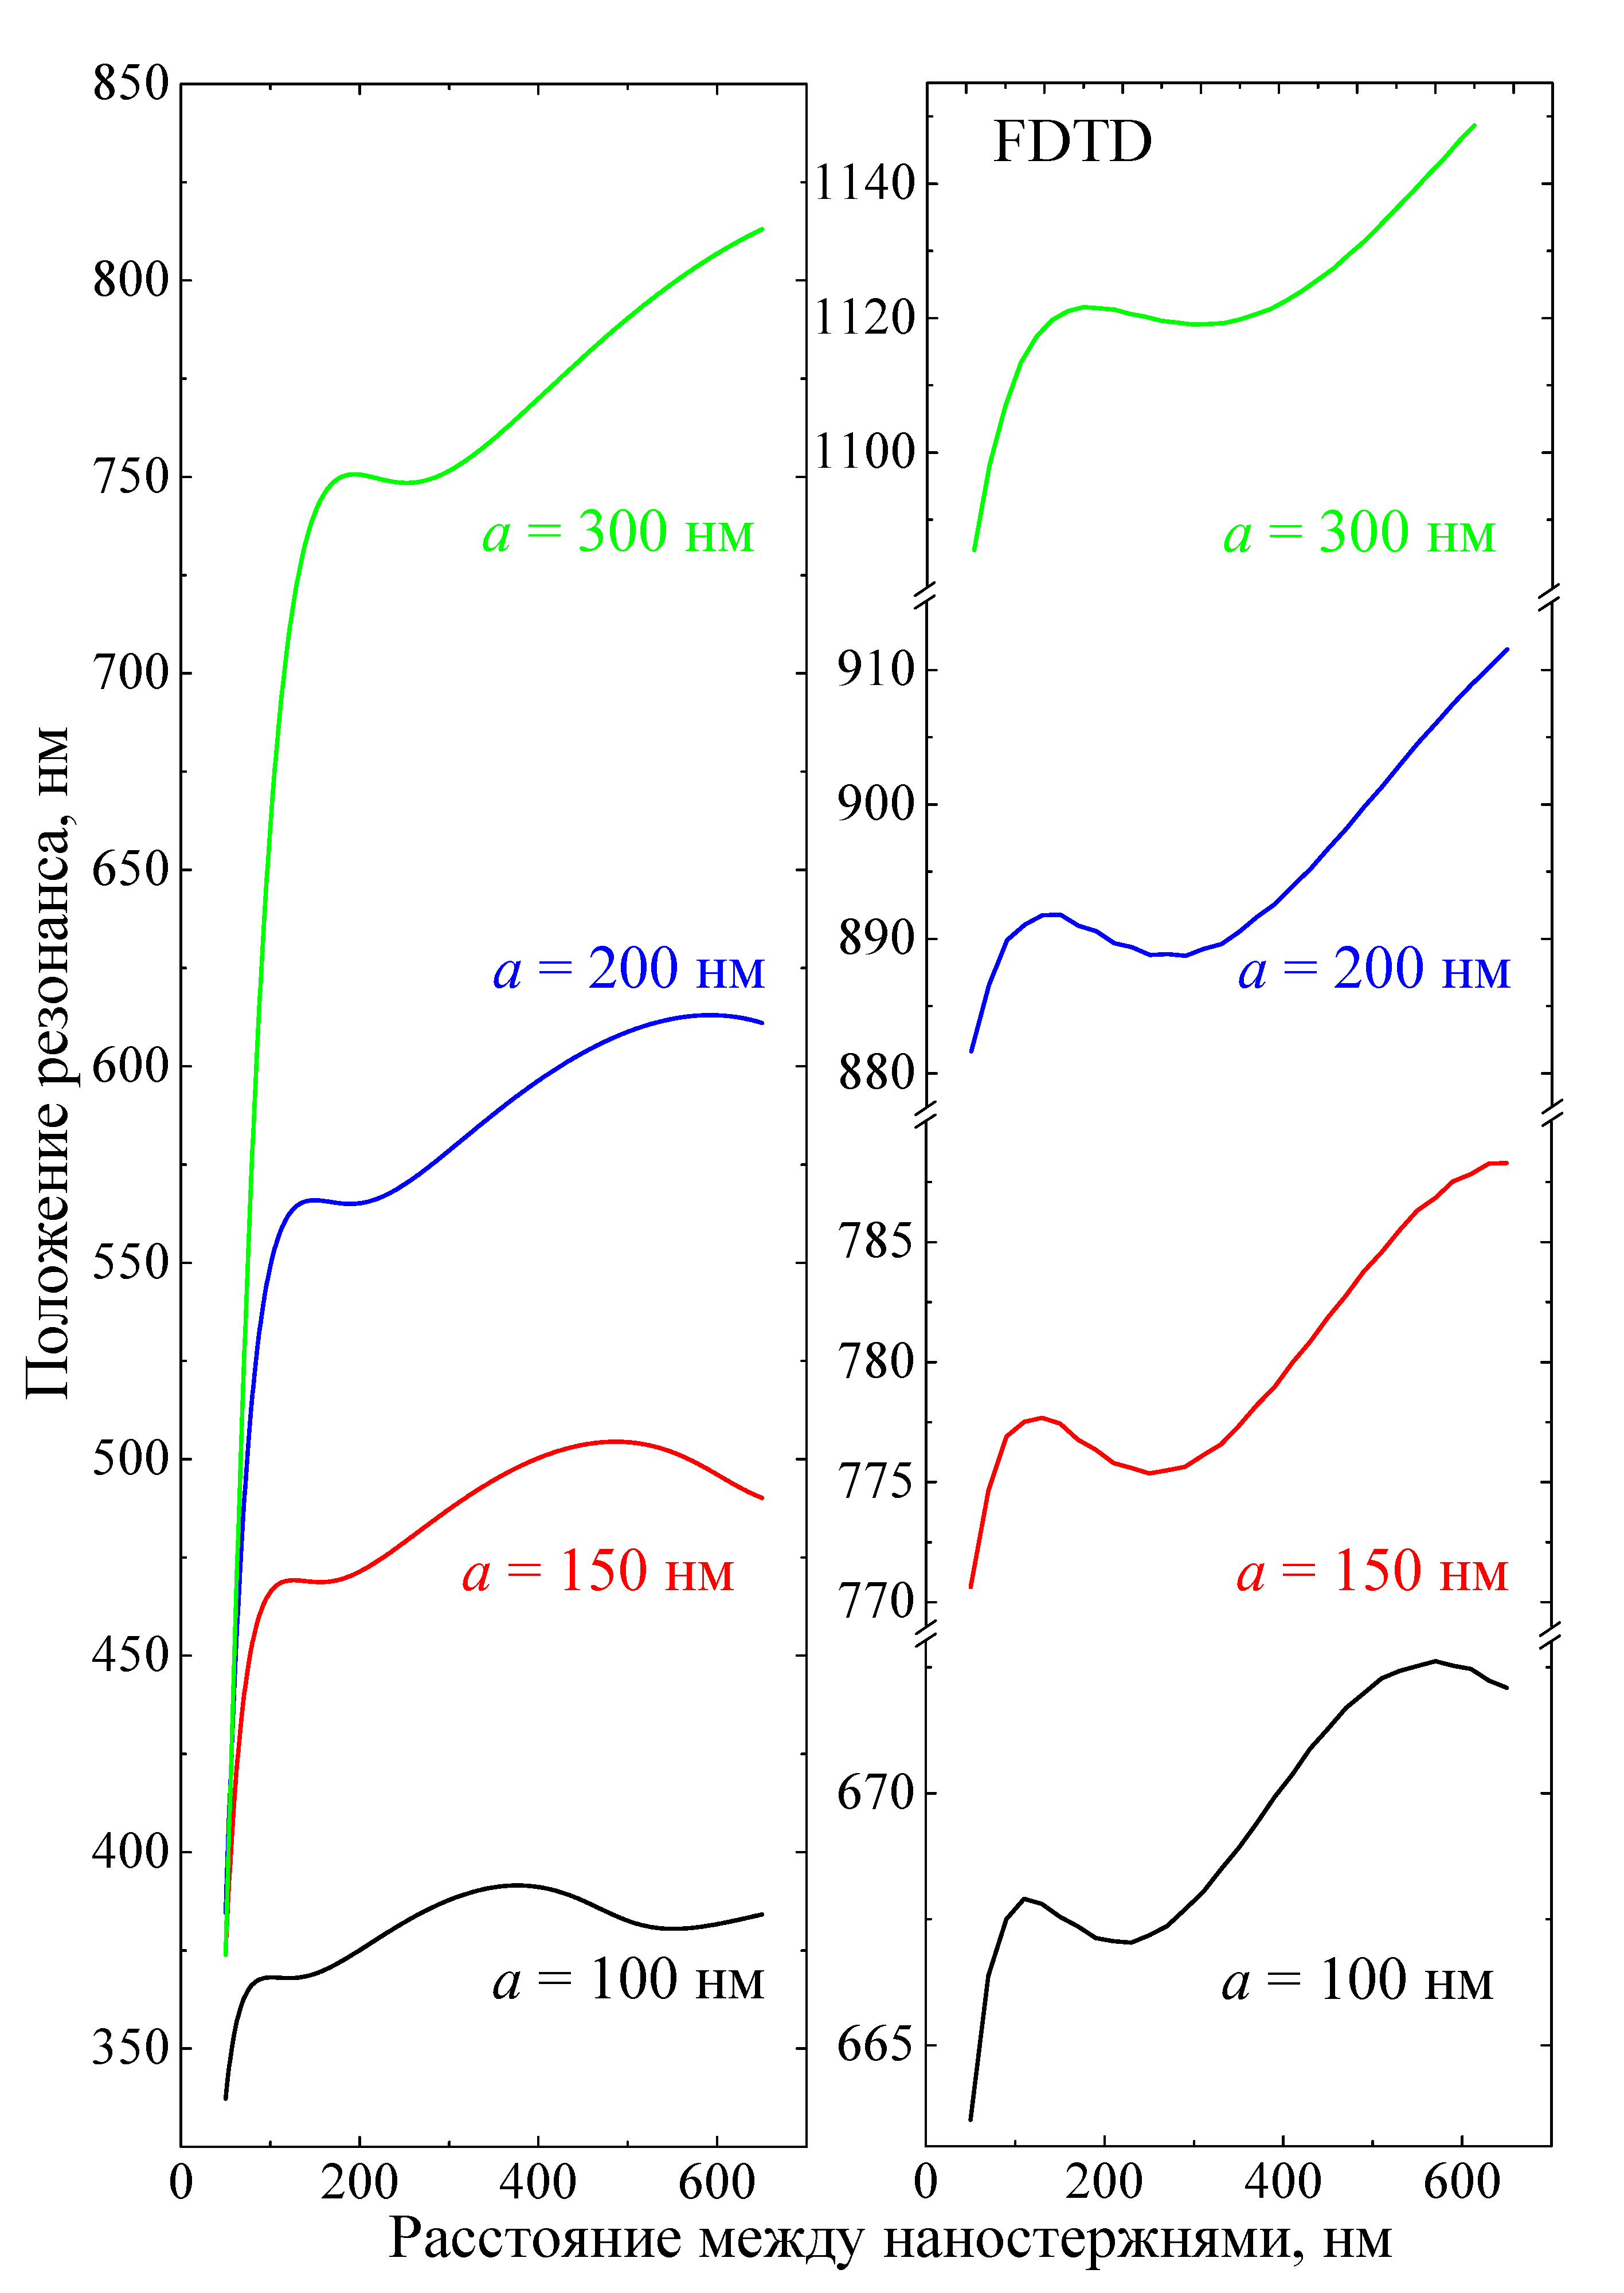
\includegraphics[width=0.6\linewidth]{img/analytics/res1_analytic_FDTD.pdf}}
\caption{Зависимость положения симметричной $ \omega_s $ и антисимметричной $ \omega_a $ резонансных частот от расстояния $ d $ между диполями.}
\label{img:res1_analytic_FDTD}
\end{figure}
Как в аналитических, так и в численных расчетах видны осцилляции. Эти осцилляции связаны дальнепольным взаимодействием эллипсоидов. Кроме того, период этих осцилляций увеличивается с увеличением длины эллипсоидов в случае аналитического расчета и с увеличением длины наностержней в случае численного расчета. 